\documentclass[aps,prd,onecolumn,nofootinbib,superscriptaddress]{revtex4-2}

\usepackage[utf8]{inputenc}
\usepackage[T1]{fontenc}
\usepackage{lmodern}
\usepackage{amsmath,amssymb,amsfonts,bm}
\usepackage{graphicx}
\usepackage{xcolor}
\usepackage{hyperref}
\usepackage{siunitx}
\usepackage{enumitem}

\hypersetup{colorlinks=true,linkcolor=blue,citecolor=blue,urlcolor=blue}

\newcommand{\Mpl}{M_{\rm Pl}}
\newcommand{\Meff}{M_{\rm eff}}
\newcommand{\dd}{\mathrm{d}}
\newcommand{\trm}{\mathrm}

\begin{document}

\title{TCV-$\phi$ V: cohesive quantum microstructure from CC-$\Phi_1$ \\
and a controlled bridge to CC-$\Phi_2$ flavour templates}

\author{Cyrille LECROQ}
\affiliation{Independent Researcher}

\date{\today}

\begin{abstract}
This fifth paper develops the quantum-microstructure layer of the canonical TCV-$\phi$ programme.
Our scope is to formulate a reproducible CC-$\Phi_1$ cluster framework, quantify its curvature response, and connect it to coarse-grained effective quantities used in previous papers.
For the flavour bridge, the historical twisted-torus benchmark is retained as the geometry that first exposed the relevance of non-trivial topology, while an extended scan within the same topological class now identifies twisted-multi-ring as the strongest current exploratory candidate.
No complete theory-level fit is claimed.
All claims are restricted to script-backed diagnostics archived in the Paper~V workspace.
\end{abstract}

\maketitle

\section{Introduction}
Paper~V follows Papers~I--IV and keeps the same canonical EFT field content and notation.
The focus is the microscopic cohesive layer (CC-$\Phi_1$) and its controlled link to exploratory CC-$\Phi_2$ flavour templates.
In this revision, the flavour subsection is organized around geometry selection:
we first compare several cluster topologies with the same PMNS-oriented criteria, then refine the leading topological family and promote the strongest resulting candidate to the primary exploratory benchmark.

\section{Canonical EFT baseline}
We keep exactly the same action and parameter hierarchy as in Papers~I--IV.
No new fundamental fields or couplings are introduced in this paper.

\section{Local CC-$\Phi_1$ clusters: setup}
We adopt a minimal cluster quantization toy consistent with the CC-$\Phi_1$ preprint construction of Ref.~\cite{TCV9}:
\begin{equation}
L_c(R)\sim \frac{1}{m_{\rm eff}(R)},
\qquad
m_{\rm eff}^2(R)=m_1^2+\xi_0 R,
\end{equation}
and
\begin{equation}
\Xi_n(R)=m_{\rm eff}^2(R)+\left(\frac{n\pi}{L_c(R)}\right)^2.
\end{equation}
Here $\Xi_n$ has mass-squared units, while the corresponding mode energy scale is
\begin{equation}
\omega_n(R)=\sqrt{\Xi_n(R)}.
\end{equation}
The baseline benchmark used by \texttt{compute\_ccphi1\_spectrum.py} is
$m_1=10^{-8}$, $\xi_0=0.1$, and $n_{\rm modes}=3$.

\section{CC-$\Phi_1$ spectrum and curvature response}
From \texttt{ccphi1\_spectrum.json}, the baseline values at $R=0$ are
\begin{equation}
 \Xi_1\simeq 1.09\times10^{-15},
\qquad
\Xi_2-\Xi_1\simeq 2.96\times10^{-15},
\end{equation}
which corresponds to $\omega_1(0)\simeq 3.30\times10^{-8}$ and coherence length
$L_c(0)\simeq 10^8$ in Planck units.
The curvature scan (\texttt{compute\_ccphi1\_curvature\_response.py}) uses
$0\le R\le 2\times10^{-15}$ and yields
\begin{equation}
\frac{\Xi_1(R)}{\Xi_1(0)}\in[1,3],
\qquad
\frac{L_c(R)}{L_c(0)}\in[0.577,1].
\end{equation}

\begin{figure}[t]
  \centering
  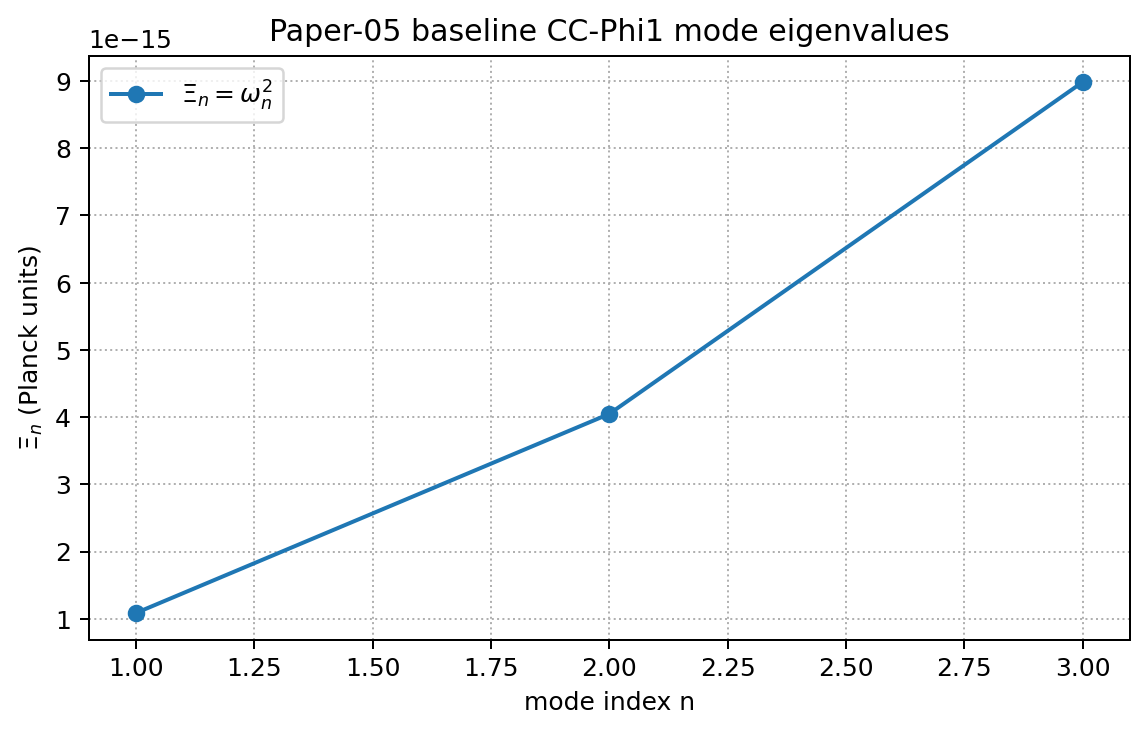
\includegraphics[width=0.72\textwidth]{../figs/ccphi1_mode_spectrum.png}
  \caption{Baseline CC-$\Phi_1$ mode spectrum from \texttt{compute\_ccphi1\_spectrum.py}.}
  \label{fig:paper5-spectrum}
\end{figure}

\begin{figure}[t]
  \centering
  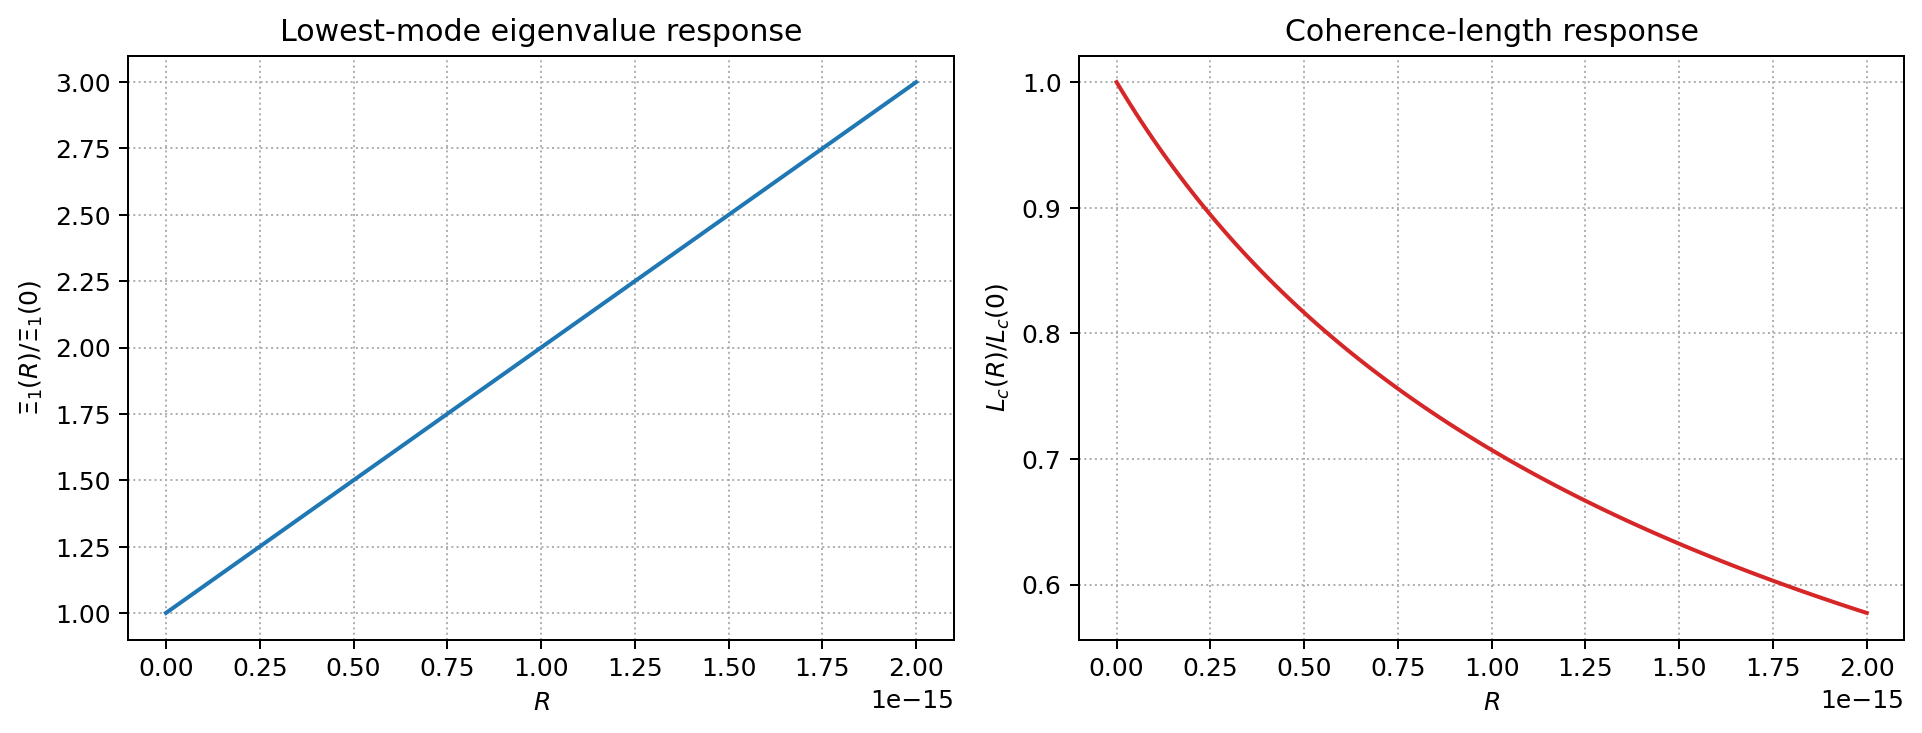
\includegraphics[width=0.86\textwidth]{../figs/ccphi1_curvature_response.png}
  \caption{Curvature response of the lowest mode and coherence length from \texttt{compute\_ccphi1\_curvature\_response.py}.}
  \label{fig:paper5-curvature}
\end{figure}

\section{Coarse-graining and effective macroscopic consistency}
At the current toy level we use a proxy density $n_{\rm CC}\sim m_1^3$ and define
\begin{equation}
\rho_{\rm cc,eff}\sim n_{\rm CC}\,\omega_1,
\qquad
p_{\rm proxy}=w_{\rm proxy}\rho_{\rm cc,eff},
\end{equation}
with the illustrative closure choice $w_{\rm proxy}=-1/2$ in the current script benchmark.
This $w_{\rm proxy}$ is a toy coarse-graining parameter and should not be interpreted as the final EFT vacuum equation of state.
The script \texttt{compute\_ccphi1\_coarse\_grain.py} gives
\begin{equation}
\rho_{\rm cc,eff}\in[3.30,5.71]\times10^{-32},
\end{equation}
over the same curvature window.
These values are used as consistency diagnostics, not as a final microscopic QFT derivation.

\begin{figure}[t]
  \centering
  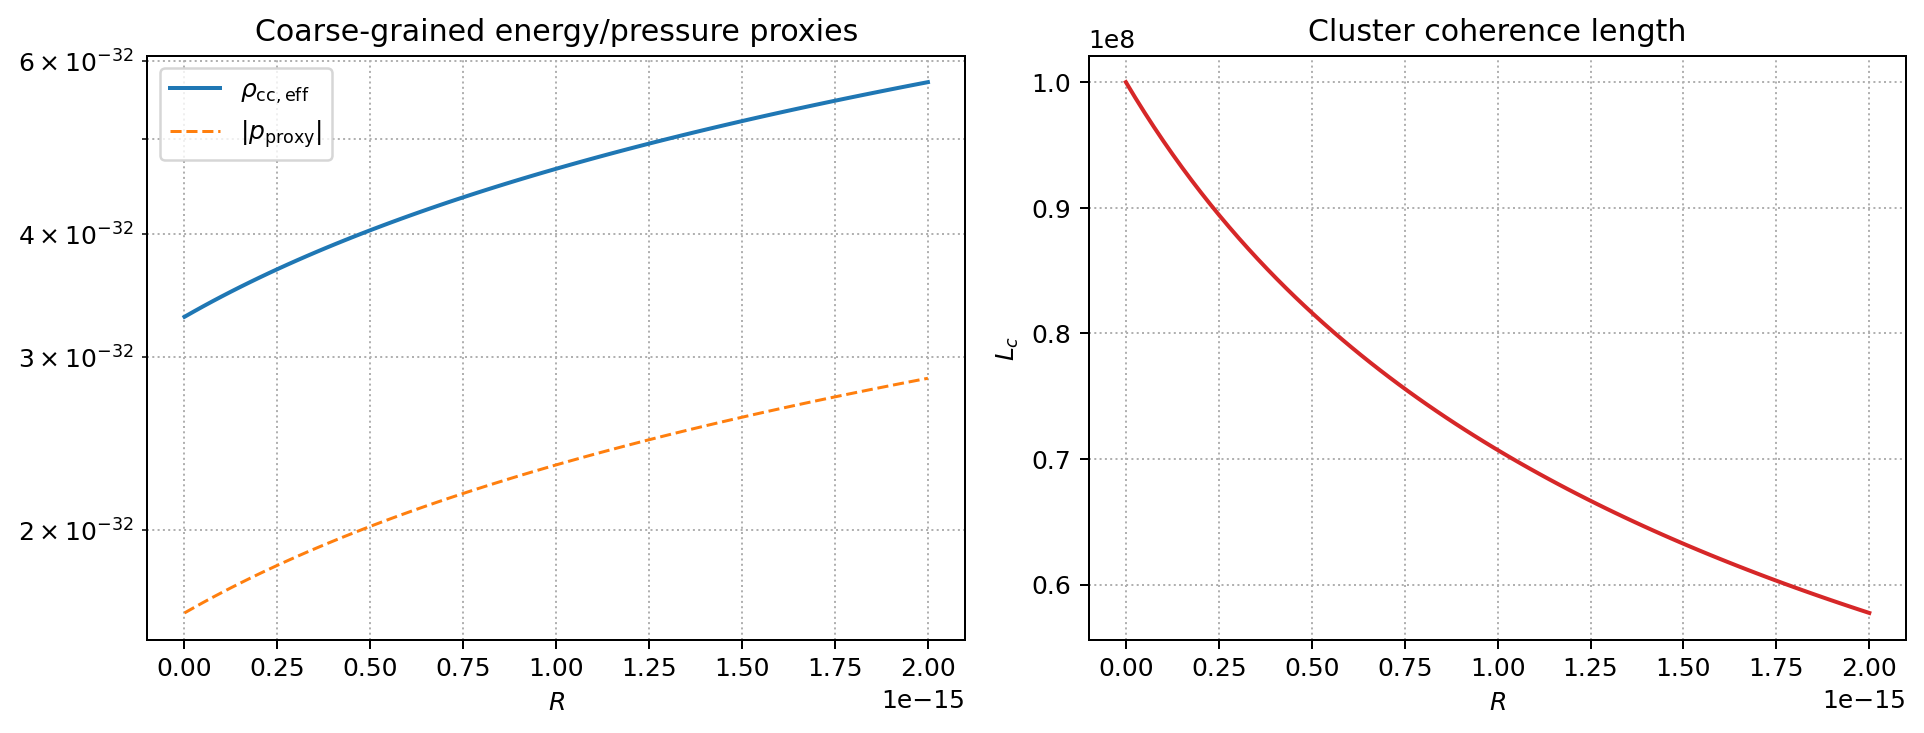
\includegraphics[width=0.86\textwidth]{../figs/ccphi1_coarse_grain.png}
  \caption{Toy coarse-graining diagnostics from \texttt{compute\_ccphi1\_coarse\_grain.py}.}
  \label{fig:paper5-coarse}
\end{figure}

\section{Exploratory bridge to CC-$\Phi_2$ flavour sector: from twisted torus to twisted multi ring}
We keep the same conservative status as in previous drafts:
this is an exploratory toy layer, not a precision global fit.
The central update is geometric.
Instead of using a single fixed cluster ansatz, we now distinguish between a historical and a current benchmark.
The twisted-torus (M\"obius-ladder) cluster remains the geometry that first produced a convincing PMNS-like signal under a common protocol.
However, a dedicated follow-up scan within the same closed twisted-topology family points to a twisted-multi-ring cluster as the stronger current flavour candidate.

The effective flavour extraction remains in the same form,
\begin{equation}
M_\ell=\mathrm{diag}(m_e,m_\mu,m_\tau)+\delta M_\ell,\qquad
M_\nu=\mathrm{diag}(m_{\nu_1},m_{\nu_2},m_{\nu_3})+\delta M_\nu,
\end{equation}
with
\begin{equation}
U_{\rm PMNS}=U_\ell^\dagger U_\nu.
\end{equation}
The key difference is that $\delta M_\ell$ and $\delta M_\nu$ are no longer tied to a single legacy template.
The initial topology-aware benchmark is generated from twisted-torus mode structure in \texttt{compute\_twisted\_torus\_flavor\_toy.py}, and the refined benchmark is generated from \texttt{compute\_twisted\_multi\_ring\_flavor\_toy.py}.
The integer parameter \texttt{twist\_shift} controls the staggered cross-channel offset between neighbouring rings; the best current candidate uses $\texttt{twist\_shift}=1$.

For the best script-backed twisted-multi-ring benchmark we obtain
\begin{equation}
\theta_{12}\simeq 32.1^\circ,\quad
\theta_{13}\simeq 7.76^\circ,\quad
\theta_{23}\simeq 45.3^\circ,
\end{equation}
with a common PMNS proximity score $S_{\rm PMNS}\simeq 0.24$ (lower is better in our normalization).
The PMNS reference point used in this toy score is
$\theta_{12}^{\rm ref}=33.0^\circ$, $\theta_{13}^{\rm ref}=8.6^\circ$,
$\theta_{23}^{\rm ref}=45.0^\circ$, consistent with current global-fit
central values (\cite{NuFIT}).
In the same scan,
\begin{equation}
n_{\rm strict}=164,\qquad n_{\rm relaxed}=285,
\end{equation}
for $n_{\rm natural}=3949$ accepted points.
For comparison, the historical twisted-torus benchmark gave
\begin{equation}
\theta_{12}\simeq 34.6^\circ,\quad
\theta_{13}\simeq 8.29^\circ,\quad
\theta_{23}\simeq 41.6^\circ,
\end{equation}
with $S_{\rm PMNS}\simeq 0.52$ and $82/4223$ strict points.
The dedicated twisted-multi-ring follow-up therefore improves both the common PMNS score and the strict-yield fraction without changing the canonical EFT field content.
The reactor angle $\theta_{13}$ lies below the current experimental central value in the best twisted-multi-ring candidate, but remains inside the strict window and is therefore consistent with the exploratory status of this benchmark.
This remains an exploratory indication of geometric viability, not a final flavour solution.

\begin{figure}[t]
  \centering
  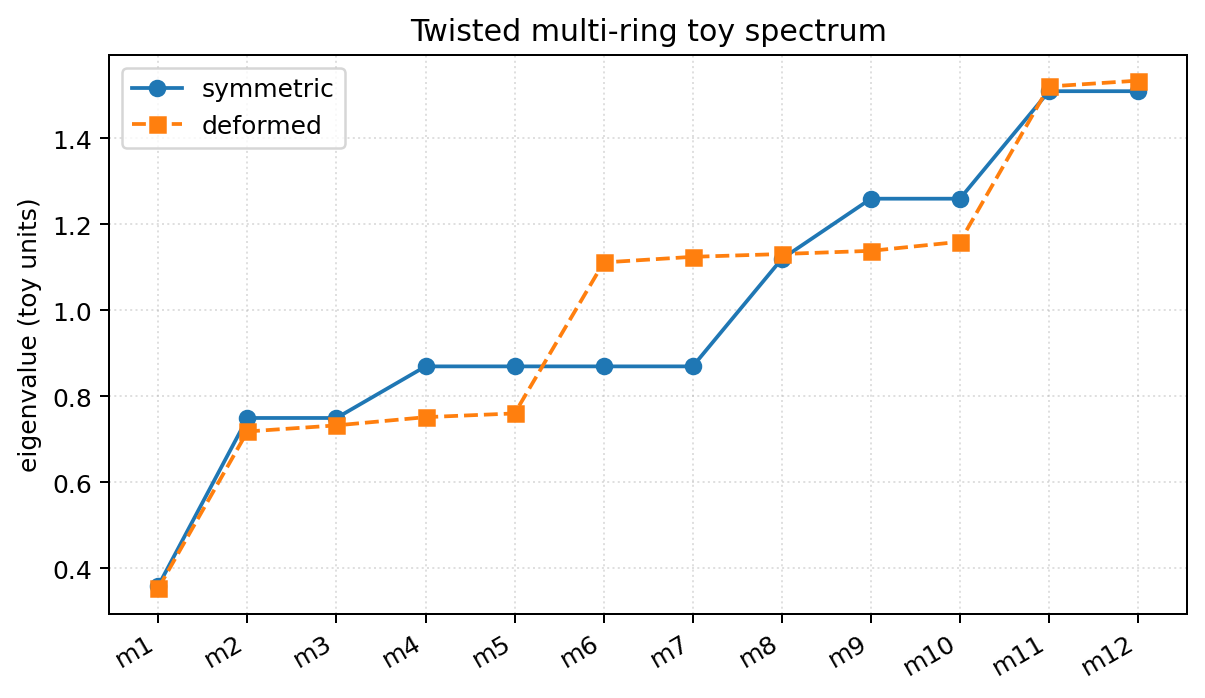
\includegraphics[width=0.68\textwidth]{../figs/twisted_multi_ring_flavour_spectrum.png}
  \caption{Twisted-multi-ring flavour spectrum from \texttt{compute\_twisted\_multi\_ring\_flavor\_toy.py}.}
  \label{fig:paper5-twisted-spectrum}
\end{figure}

\begin{figure}[t]
  \centering
  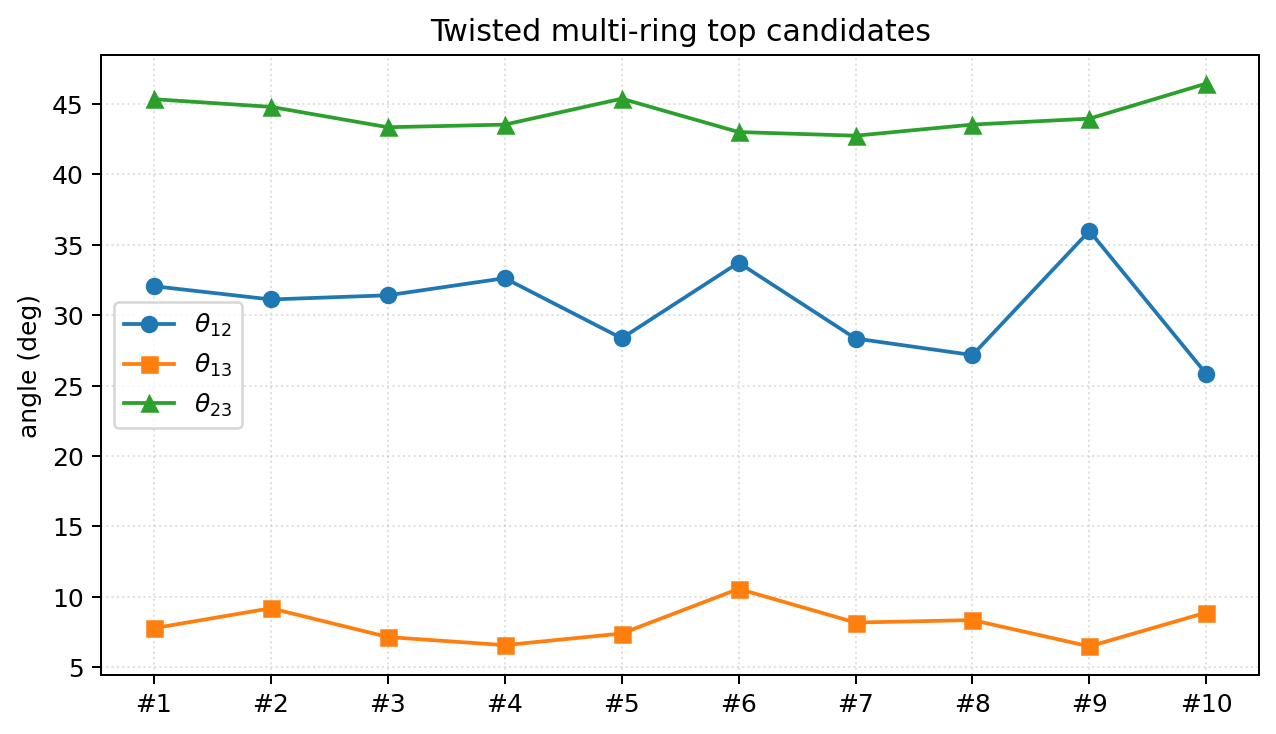
\includegraphics[width=0.68\textwidth]{../figs/twisted_multi_ring_flavour_top_candidates.png}
  \caption{Top twisted-multi-ring flavour candidates (script-backed).}
  \label{fig:paper5-twisted-candidates}
\end{figure}

\section{Geometric exploration and model selection diagnostics}
To avoid hidden fine tuning, we compare candidate geometries under a common protocol:
same angle windows, same naturalness bounds, and the same normalized PMNS score used across all toys.
The aggregate diagnostics are produced by \texttt{compute\_flavour\_geometry\_comparison.py}.
The score is defined as
\begin{equation}
S_{\rm PMNS}=
\sqrt{
\left(\frac{\theta_{12}-33^\circ}{10^\circ}\right)^2+
\left(\frac{\theta_{13}-8.6^\circ}{4^\circ}\right)^2+
\left(\frac{\theta_{23}-45^\circ}{7^\circ}\right)^2
},
\end{equation}
and is combined with strict-yield fractions into a PMNS viability index in the summary JSON.

\begin{table}[t]
  \centering
  \begin{tabular}{lccc}
    \hline\hline
    Geometry & Representative score $S_{\rm PMNS}$ & Strict yield within natural scan & PMNS viability index \\
    \hline
    Pyramidal & 2.40 & --- (single benchmark) & 0.067 \\
    Tetrahedral apex/base & 2.23 & $0/1500$ & 0.107 \\
    Tetrahedral star & 2.64 & $0/2701$ & 0.013 \\
    Torus ring & 0.78 & $59/4358$ & 0.448 \\
    Spherical shell & 2.69 & $0/4348$ & 0.000 \\
    Twisted torus & 0.52 & $82/4223$ & 0.510 \\
    \hline\hline
  \end{tabular}
  \caption{Initial cross-geometry exploratory comparison from \texttt{flavour\_geometry\_comparison\_summary.json}.}
  \label{tab:paper5-geometry-comparison}
\end{table}

\begin{figure}[t]
  \centering
  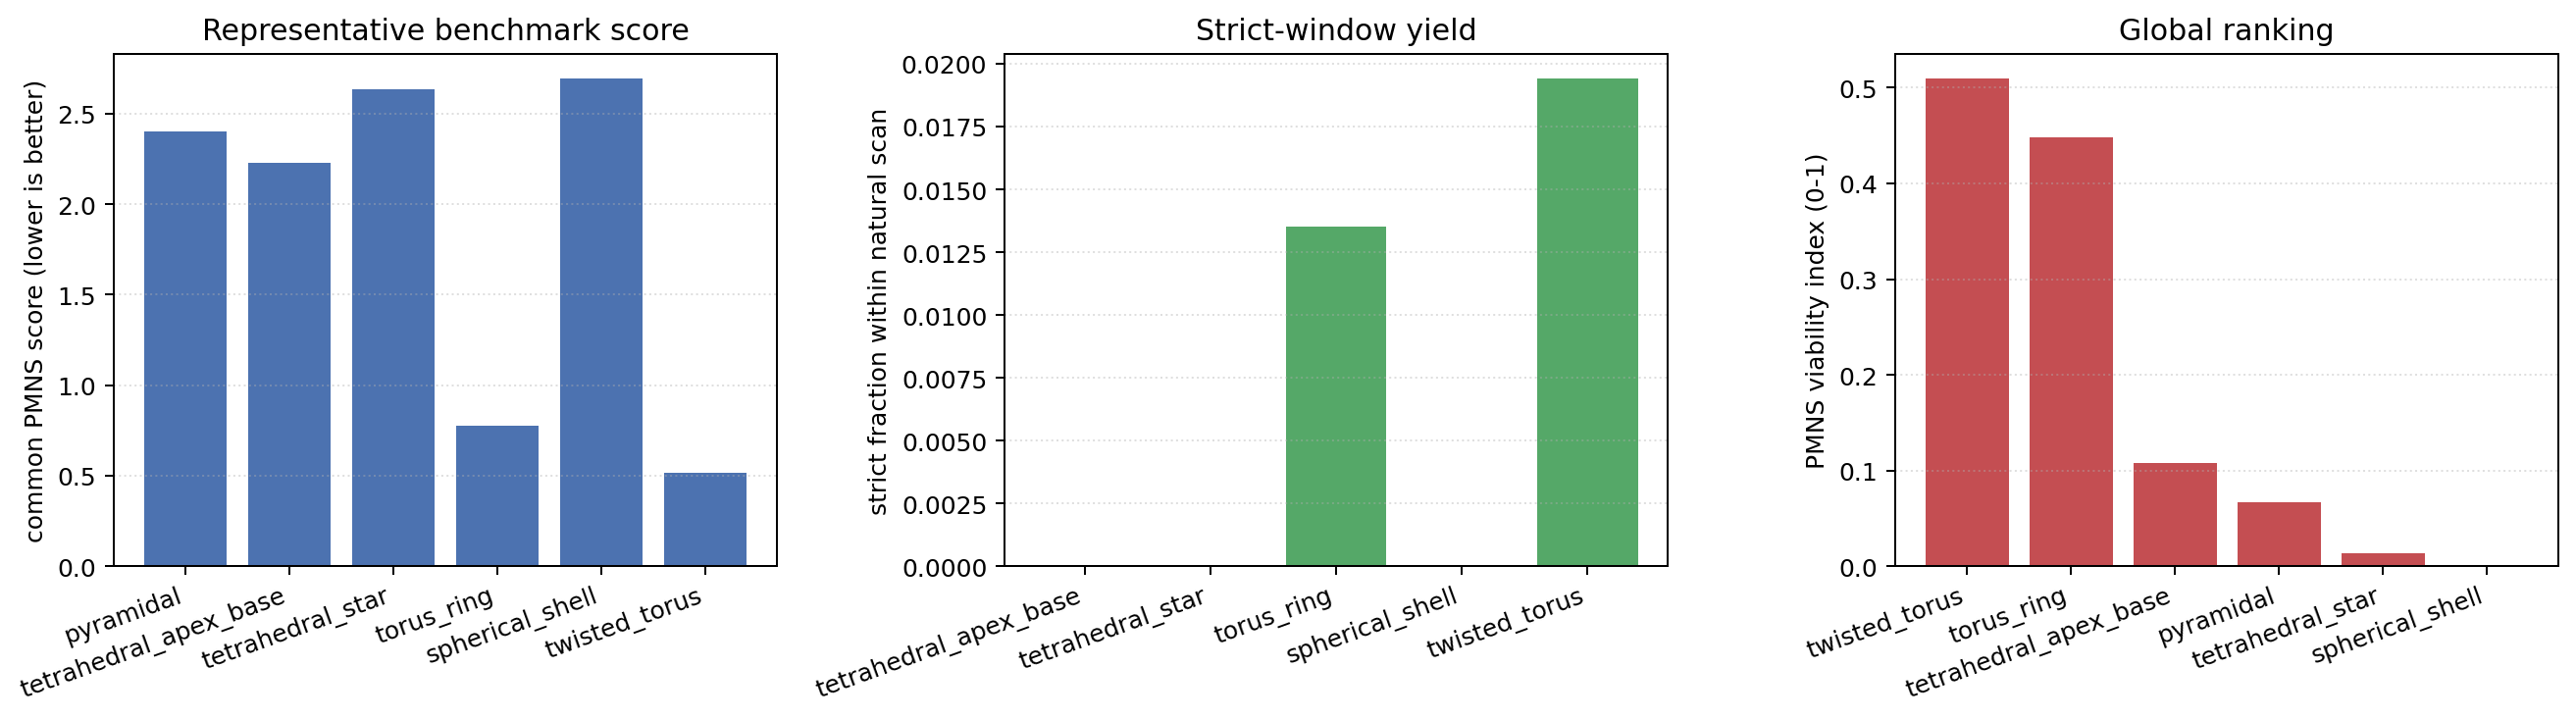
\includegraphics[width=0.92\textwidth]{../figs/flavour_geometry_comparison_overview.png}
  \caption{Common-score and strict-yield comparison across explored cluster geometries.}
  \label{fig:paper5-geometry-overview}
\end{figure}

The main conclusion of this initial comparison is limited and explicit:
within the current exploratory setup, topologically non-trivial geometries (torus ring and twisted torus) produce non-zero strict-window populations in large scans, while the tested rigid geometries (pyramidal, tetrahedral, spherical) remain at zero strict hits.
This is the step that first singled out twisted-torus as the correct family direction.
An intermediate phase-loop toy was also tested in the same spirit, but its dedicated flavour benchmark remained clearly below the twisted-torus and twisted-multi-ring results, so it is retained only as a superseded exploratory waypoint in the archived workspace.

We then refine this direction with a dedicated same-family comparison between twisted torus and twisted multi ring.
The diagnostics are stored in \texttt{twisted\_multi\_ring\_vs\_twisted\_torus\_comparison.json}.

\begin{table}[t]
  \centering
  \begin{tabular}{lcc}
    \hline\hline
    Candidate & $S_{\rm PMNS}$ & Strict fraction within natural scan \\
    \hline
    Twisted torus & 0.519 & 0.0194 \\
    Twisted multi ring & 0.235 & 0.0415 \\
    \hline\hline
  \end{tabular}
  \caption{Dedicated PMNS-level comparison within the leading twisted-topology family.}
  \label{tab:paper5-twisted-headtohead}
\end{table}

The dedicated twisted-multi-ring benchmark improves the twisted-torus score by roughly a factor of two and doubles the strict-yield fraction.
In the logic of this paper, twisted torus remains the historical turning point, but twisted multi ring becomes the strongest current PMNS candidate.

\section{Sector-compatibility stress tests for twisted multi ring}
We then test whether the same twisted-multi-ring geometry remains compatible with a hierarchical charged-lepton sector and with a weak-mixing quark-like toy sector.
The diagnostics are generated by \texttt{compute\_twisted\_multi\_ring\_sector\_compatibility.py}.

For charged leptons, perturbing the charged-sector controls around the best twisted-multi-ring point yields
\begin{equation}
f_{\rm strict}^{(\ell)}\simeq 0.87,
\end{equation}
i.e. approximately $87\%$ of tested points remain in the strict PMNS window.
This is stronger than the historical twisted-torus robustness level ($\sim 70\%$) and therefore supports the same candidate shift seen in the PMNS benchmark itself.
For the quark-like toy layer, the mean mixing angles stay small,
\begin{equation}
\langle \theta_{12}^{q}\rangle\simeq 0.35^\circ,\quad
\langle \theta_{13}^{q}\rangle\simeq 1.2\times10^{-3}\,^\circ,\quad
\langle \theta_{23}^{q}\rangle\simeq 2.0\times10^{-3}\,^\circ.
\end{equation}
These tests support compatibility at the toy level, but do not constitute a complete SM flavour derivation.

\begin{figure}[t]
  \centering
  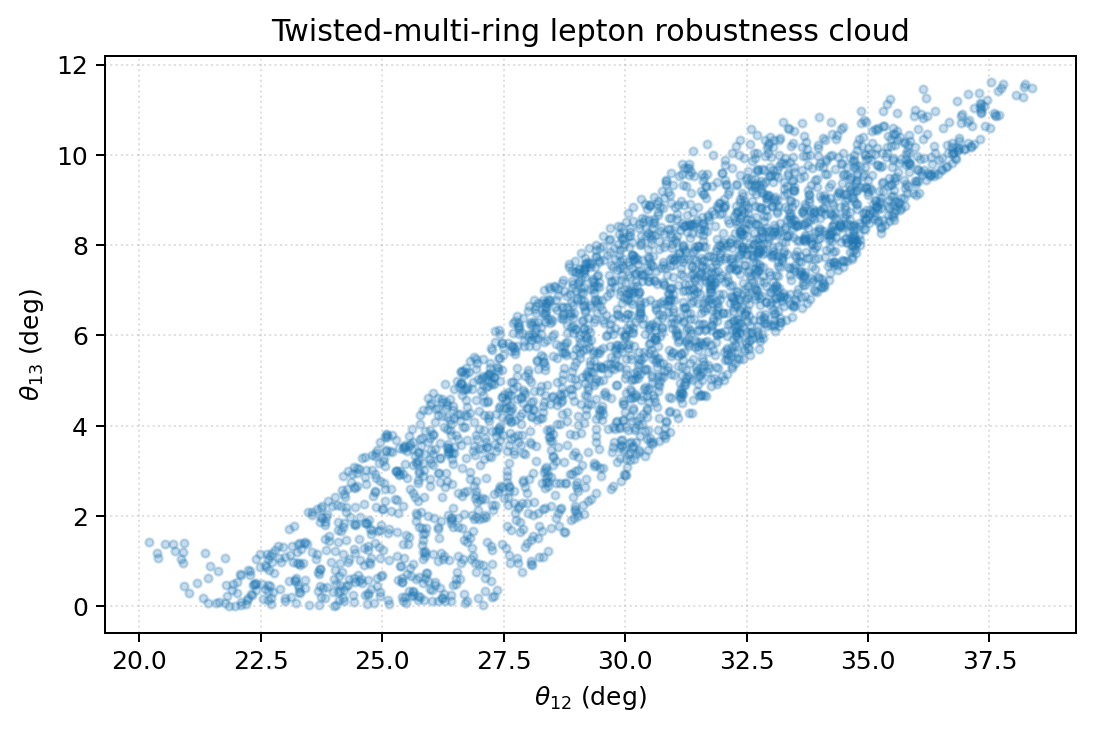
\includegraphics[width=0.70\textwidth]{../figs/twisted_multi_ring_lepton_robustness_cloud.png}
  \caption{Twisted-multi-ring lepton robustness cloud from \texttt{compute\_twisted\_multi\_ring\_sector\_compatibility.py}.}
  \label{fig:paper5-twisted-dashboard}
\end{figure}

\begin{figure}[t]
  \centering
  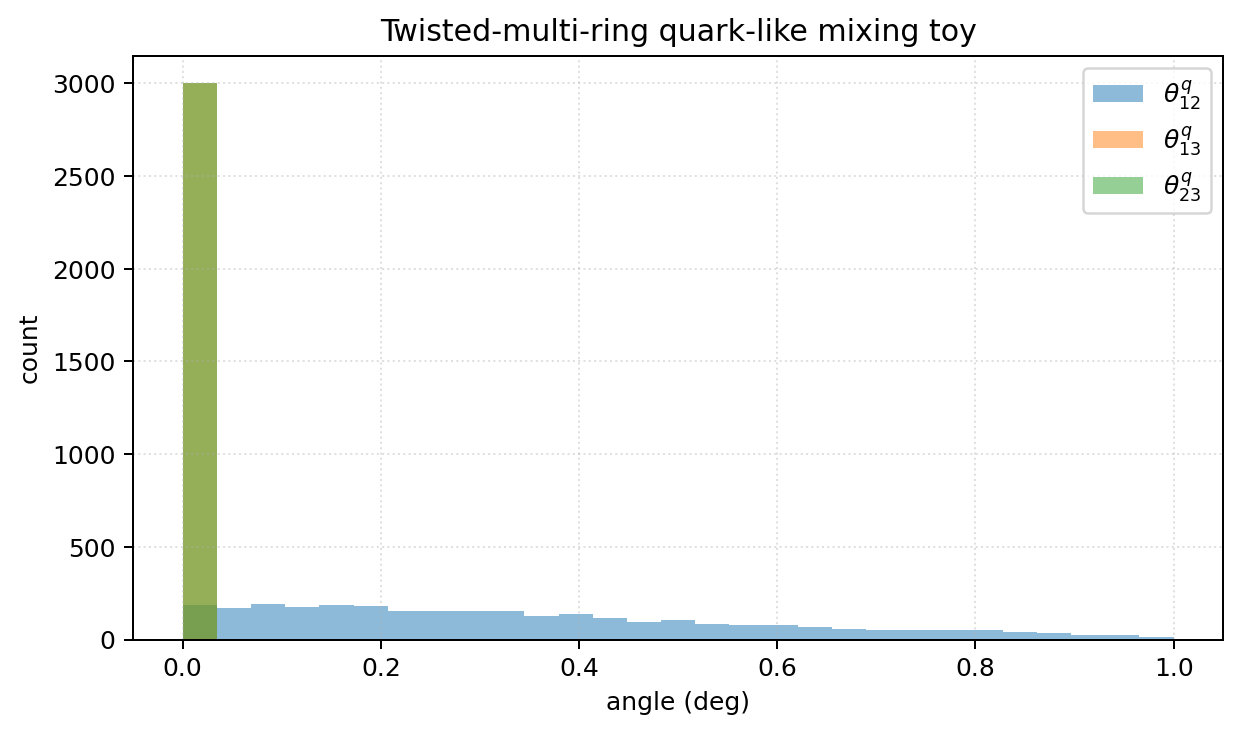
\includegraphics[width=0.70\textwidth]{../figs/twisted_multi_ring_quark_like_hist.png}
  \caption{Twisted-multi-ring quark-like toy mixing distribution. The angles remain small and hierarchical in this exploratory layer.}
  \label{fig:paper5-twisted-quark}
\end{figure}

\begin{table}[t]
  \centering
  \begin{tabular}{lcc}
    \hline\hline
    Block & Output artifact & Status label \\
    \hline
    CC-$\Phi_1$ spectrum & \texttt{ccphi1\_spectrum.json} & phenomenological toy \\
    Curvature response & \texttt{ccphi1\_curvature\_scan.npz} & phenomenological scan \\
    Coarse-graining & \texttt{ccphi1\_coarse\_grain.json} & toy proxy \\
    Legacy pyramidal flavour toy & \texttt{ccphi2\_flavour\_toy.json} & exploratory legacy benchmark \\
    Twisted-torus flavour toy & \texttt{twisted\_torus\_flavour\_toy\_summary.json} & exploratory historical benchmark \\
    Phase-loop flavour toy & \texttt{phase\_loop\_flavour\_toy\_summary.json} & exploratory intermediate, superseded \\
    Twisted-multi-ring flavour toy & \texttt{twisted\_multi\_ring\_flavour\_toy\_summary.json} & exploratory current benchmark \\
    Geometry comparison & \texttt{flavour\_geometry\_comparison\_summary.json} & exploratory selection diagnostic \\
    Twisted-family head-to-head & \texttt{twisted\_multi\_ring\_vs\_twisted\_torus\_comparison.json} & exploratory refinement diagnostic \\
    Sector compatibility & \texttt{twisted\_multi\_ring\_sector\_compatibility\_summary.json} & exploratory stress test \\
    \hline\hline
  \end{tabular}
  \caption{Paper-V script-backed outputs and status labels.}
  \label{tab:paper5-status}
\end{table}

\section{Status of assumptions}
\begin{itemize}
  \item EFT-derived baseline definitions inherited from Papers~I--IV.
  \item Phenomenological closures used in the CC-$\Phi_1$ cluster pipeline.
  \item Exploratory geometry-to-flavour mapping for CC-$\Phi_2$.
  \item Twisted-torus identified as the historical topology that opened the correct PMNS direction.
  \item Twisted-multi-ring selected as the strongest current exploratory flavour candidate, without changing the canonical EFT.
\end{itemize}

\section{Conclusion}
Paper~V is designed as a reproducible and conservative microstructure step in the TCV-$\phi$ series.
Relative to earlier drafts, the flavour bridge is now organized as a geometry-selection problem:
we test multiple cluster topologies under common criteria, identify twisted torus as the historical turning point, and then show that a refined twisted-multi-ring geometry becomes the strongest current exploratory candidate.
This improves the naturalness narrative at the toy level while keeping all macro-level sectors (bounce, black holes, and cosmological fits) unchanged in this paper.
A full micro-to-macro closure from this topological family is left for future work.

\begin{thebibliography}{99}

\bibitem{TCV1}
C.~Lecroq, ``TCV-$\phi$ I: an effective cohesive--vacuum field theory and its $\Lambda$CDM-compatible background cosmology,'' preprint (2026), \href{https://doi.org/10.5281/zenodo.19234640}{zenodo.19234640}.

\bibitem{TCV2}
C.~Lecroq, ``TCV-$\phi$ II: cohesive bounce, geometric reheating, and baseline baryogenesis/ULDM pipelines,'' preprint (2026), \href{https://doi.org/10.5281/zenodo.19234953}{zenodo.19234953}.

\bibitem{TCV3}
C.~Lecroq, ``TCV-$\phi$ III: primordial perturbations across the cohesive bounce and CLASS/CAMB bridge diagnostics,'' preprint (2026), \href{https://doi.org/10.5281/zenodo.192355333}{zenodo.192355333}.

\bibitem{TCV4}
C.~Lecroq, ``TCV-$\phi$ IV: cohesive non-singular black holes from static cores to slow rotation in the canonical EFT,'' preprint (2026), \href{https://doi.org/10.5281/zenodo.19235896}{zenodo.19235896}.

\bibitem{NuFIT}
I.~Esteban \textit{et al.}, ``NuFIT 5.x global fit of neutrino oscillation parameters,'' online resource (accessed 2026), \url{https://www.nu-fit.org/}.

\end{thebibliography}

\end{document}
